\documentclass{beamer}
\usepackage[utf8]{inputenc}
\usepackage[T1]{fontenc}
\usepackage[brazilian]{babel}
\usepackage{lmodern}
\usetheme{default}
\usecolortheme{beaver}
\usepackage{graphicx,xcolor}
\usepackage{amsmath}


\newcommand{\sen}{\operatorname{sen}}
\newtheorem{definicao}[theorem]{Definição}
\newtheorem{teorema}[theorem]{Teorema}
\newtheorem{solucao}[theorem]{Solução}
\beamertemplatenavigationsymbolsempty

\makeatletter
\def\th@mystyle{%
	\ttfamily 
	\setbeamercolor{block title example}{bg=red!30,fg=black}
	\setbeamercolor{block body example}{bg=red!10,fg=black!80}
	\def\inserttheoremblockenv{exampleblock}
}
\makeatother
\theoremstyle{mystyle}
\newtheorem{algoritmo}[theorem]{Algoritmo}

\title{Integração Numérica}
\author
{
	Prof. Jonathan Esteban Arroyo Silva	
}
\institute
{
	Departamento de Ciência da Computação\\
	Universidade Federal de São João del-Rei\\
	\texttt{silva.jea@ufsj.edu.br}
}
\date{}
\logo{\includegraphics[width=0.2\linewidth]{../ufsj-logo-site}}

\begin{document}
	
\begin{frame}[plain]
    \maketitle
\end{frame}

\begin{frame}[plain]
	\frametitle{Sumário}
	\tableofcontents
\end{frame}

\section{Introdução}
	\begin{frame}
		\frametitle{Introdução}	
		Como o nome sugere, estamos interessados em estudar métodos numéricos para calcular de forma aproximada a integral de uma função com uma variável real em um intervalo $ [a, b] $:
		\begin{equation*}
			I = I(f) = \int_{a}^{b} f(x) dx
		\end{equation*}
		sendo $ f (x) $ uma função contínua com derivadas contínuas no intervalo [a, b].
	\end{frame}

	\begin{frame}
		\frametitle{Introdução}	
		Pelo Teorema Fundamental do Cálculo, sabemos que:
		\begin{equation*}
			I = \int_{a}^{b} f(x) dx = F(b) - F(a)
		\end{equation*}
		sendo $ F (x) $ a função primitiva de $ f (x) $, tal que $ F ^{\prime}(x) = f (x) $.
	\end{frame}

	\begin{frame}
		\frametitle{Introdução}	
		Por outro lado, é importante lembrar que a integral pode ser definida através de um somatório infinito de áreas de retângulos:
		\begin{equation*}
			I = \int_{a}^{b} f(x) dx = \sum_{i = 0}^{n = \infty} f(x_{i})(x_{i+1} - x_{i})
		\end{equation*}
		sendo $ x_{i} $ os pontos da discretização em $ x $, como no exemplo a seguir (n=5):
		\begin{figure}
			\centering
			\includegraphics[width=0.4\linewidth]{Figuras/grafico_01}
			\label{fig:grafico01}
		\end{figure}
	\end{frame}
	
	\begin{frame}
		\frametitle{Introdução}	
		De modo geral, a integração numérica consiste em integrar o polinômio $ P_{n} (x) $ que interpola os pontos:
		\begin{equation*}
			 (x_{0},f(x_{0})),(x_{1},f(x_{1})),\ldots,(x_{n},f(x_{n}))
		\end{equation*}
		sendo $ x_{0},x_{1},\ldots,x_{n}\in [a,b]  $, ou seja: 
		\begin{equation*}
			I = \int_{a}^{b} f(x) dx \approx \int_{x_{0}}^{x_{n}} P_{n}(x) dx
		\end{equation*}
		por ser mais fácil de computar e trabalhar, como comentado em aulas anteriores.
	\end{frame}

\section{Fórmulas Fechadas de Newton-Cotes}

	\begin{frame}
		\frametitle{Fórmulas Fechadas de Newton-Cotes}
		\begin{itemize}
			\item Considera-se inicialmente as fórmulas de Newton-Cotes do	tipo fechada, isto é, quando $ x_{0} = a $ e $ x_{n} = b $
			\item Serão adotados polinômios interpoladores $ P_{n} (x) $ sobre nós igualmente espaçados no intervalo $ [a, b] $
			\item Assim, $ x_{i} = \left( \dfrac{b-a}{n}\right) i + a;\;\; i = 0,1,\ldots,n  $
			\item Consequentemente, $ h = \dfrac{b-a}{n} \rightarrow x_{i} = x_{0} + ih;\;\; i = 0,1,\ldots,n  $
		\end{itemize}
	\end{frame}
	
	\begin{frame}
		\frametitle{Regra do Retângulo}
		\begin{itemize}
			\item Como o polinômio mais simples é o polinômio constante, começaremos com ele
			\item Assim, $ f (x) $ será aproximada pelo seu valor em $ x_{0} = a $ (ou em $ x_{1} = b $), de forma que:
			\begin{align*}
				\int_{a}^{b} f(x) dx \approx \int_{x_{0} = a}^{x_{n} = b} P_{n}(x) dx & = \int_{a}^{b} f(a) dx = \left. \left[ xf(a)\right] \right|_{a}^{b}\\
				& = (b-a)f(a) = hf(a)
			\end{align*}
			\begin{figure}
				\centering
				\includegraphics[width=0.4\linewidth]{Figuras/grafico_02}
				\label{fig:grafico02}
			\end{figure}
		\end{itemize}
	\end{frame}
	
	\begin{frame}
		\frametitle{Regra do Retângulo - Ponto médio}
		\begin{itemize}
			\item Escolhendo $ f (x) $ em algum outro ponto do intervalo $ [a, b] $, podemos ter um melhor resultado?
			\item Uma escolha comum é o ponto médio do intervalo
			\begin{equation*}
				\int_{a}^{b} f(x) dx \approx (b-a)f\left( \dfrac{a + b}{2}\right) = hf\left( \dfrac{a + b}{2}\right)
			\end{equation*}
			\begin{figure}
				\centering
				\includegraphics[width=0.4\linewidth]{Figuras/grafico_03}
				\label{fig:grafico03}
			\end{figure}
		\end{itemize}
	\end{frame}

	\begin{frame}
		\frametitle{Regra do Trapézio}
		Seja $ P_{1} (x) $ o polinômio interpolador de $ f (x) $ que passa pelos pontos $ (x_{0} , f (x_{0})) $ e $ (x_{1} , f (x_{1})) $, com $ x_{0} = a $ e $ x_{1} = b $, então, utilizando a forma de Lagrange para interpolação, tem-se:
		\begin{equation*}
			\int_{a}^{b} f(x) dx \approx \int_{a}^{b} P_{1}(x) dx = \int_{a}^{b} f(x_{0})L_{0}(x) + f(x_{1})L_{1}(x) dx
		\end{equation*}
	\end{frame}

	\begin{frame}
		\frametitle{Regra do Trapézio}
		Após alguns passos de algebrismo, tem-se
		\begin{equation*}
			\int_{a}^{b} P_{1}(x) dx = \dfrac{h}{2}\left( f(x_{0}) + f(x_{1}) \right) 
		\end{equation*}
		\begin{figure}
			\centering
			\includegraphics[width=0.4\linewidth]{Figuras/grafico_04}
			\label{fig:grafico04}
		\end{figure}
	\end{frame}

	\begin{frame}
		\frametitle{Exemplo}
		Calcule de forma aproximada o valor da seguinte integral $ \int_{0}^{1.2} e^{x}\cos(x) dx $ usando a regra do trapézio.
		\pause
		
		\begin{itemize}
			\item  Como $ a = x_{0} = 0 $ e $ b = x_{1} = 1.2 $, logo $ h = x_{1} - x_{0} = 1.2$
			\item  Calculando os valores da função em $ x_{0} $ e $ x_{1} $ tem-se $ f(0)  = e^{0}\cos(0) = 1 $ e $ f(1.2)  = e^{1.2}\cos(1.2) = 1.2 $
			\item Assim,
			\begin{equation*}
				\int_{0}^{1.2} e^{x}\cos(x) dx \approx \dfrac{1.2}{2}\left( 1 + 1.2 \right) = 1.32
			\end{equation*}
		\end{itemize}
	\end{frame}

	\begin{frame}
		\frametitle{Exemplo}
		\begin{figure}
			\centering
			\includegraphics[width=1.0\linewidth]{Figuras/grafico_05}
			\label{fig:grafico05}
		\end{figure}
	\end{frame}

	\begin{frame}
		\frametitle{Regra 1/3 de Simpson}
		Seja $ P_{2} (x) $ o polinômio interpolador de $ f (x) $ que passa pelos pontos $ (x_{0} , f (x_{0})) $, $ (x_{1} , f (x_{1})) $ e $ (x_{2} , f (x_{2})) $, com $ x_{0} = a $ e $ x_{2} = b $, então, utilizando a forma de Lagrange para interpolação, tem-se:
		\begin{align*}
			\int_{a}^{b} f(x) dx \approx \int_{a}^{b} P_{2}(x) dx
			&= f(x_{0})\int_{x_{0}}^{x_{2}} \dfrac{(x - x_{1})(x - x_{2})}{(x_{0} - x_{1})(x_{0} - x_{2})} dx\\
			&+ f(x_{1})\int_{x_{0}}^{x_{2}} \dfrac{(x - x_{0})(x - x_{2})}{(x_{1} - x_{0})(x_{1} - x_{2})} dx\\
			&+ f(x_{2})\int_{x_{0}}^{x_{2}} \dfrac{(x - x_{0})(x - x_{1})}{(x_{2} - x_{0})(x_{2} - x_{1})} dx
		\end{align*}
		e após alguns passos algébricos, tem-se:
		\begin{equation*}
			\dfrac{h}{3}(f(x_{0}) + 4f(x_{1}) + f(x_{2}))
		\end{equation*}
	\end{frame}
	
	\begin{frame}
		\frametitle{Exemplo}
		Calcule de forma aproximada o valor da seguinte integral $ \int_{0}^{1.2} e^{x}\cos(x) dx $ usando a regra 1/3 de Simpson.
		\pause
		
		\begin{itemize}
			\item  Como $ a = x_{0} = 0 $ e $ b = x_{2} = 1.2 $, logo $ h = \dfrac{x_{2} - x_{0}}{2} = 0.6$
			\item  Calculando os valores da função em $ x_{0} $, $ x_{1} $ e $ x_{2} $ tem-se $ f(0)  = e^{0}\cos(0) = 1 $, $ f(0.6)  = e^{0.6}\cos(0.6) = 1.5 $ e $ f(1.2)  = e^{1.2}\cos(1.2) = 1.2 $
			\item Assim,
			\begin{equation*}
				\int_{0}^{1.2} e^{x}\cos(x) dx \approx \dfrac{0.6}{3}\left( 1 + 4\cdot1.5 + 1.2 \right) = 1.64
			\end{equation*}
		\end{itemize}
	\end{frame}

	\begin{frame}
		\frametitle{Regra 3/8 de Simpson}
		Seja $ P_{3} (x) $ o polinômio interpolador de $ f (x) $ que passa pelos pontos $ (x_{0} , f (x_{0})) $, $ (x_{1} , f (x_{1})) $, $ (x_{2} , f (x_{2})) $ e $ (x_{3} , f (x_{3})) $  com $ x_{0} = a $ e $ x_{3} = b $, então, utilizando a forma de Lagrange para interpolação, tem-se:
		\begin{align*}
			\int_{a}^{b} f(x) dx \approx \int_{a}^{b} P_{3}(x) dx
			&= f(x_{0})\int_{x_{0}}^{x_{3}} \dfrac{(x - x_{1})(x - x_{2})(x - x_{3})}{(x_{0} - x_{1})(x_{0} - x_{2})(x_{0} - x_{3})} dx\\
			&+ f(x_{1})\int_{x_{0}}^{x_{3}} \dfrac{(x - x_{0})(x - x_{2})(x - x_{3})}{(x_{1} - x_{0})(x_{1} - x_{2})(x_{1} - x_{3})} dx\\
			&+ f(x_{2})\int_{x_{0}}^{x_{3}} \dfrac{(x - x_{0})(x - x_{1})(x - x_{3})}{(x_{2} - x_{0})(x_{2} - x_{1})(x_{2} - x_{3})} dx\\
			&+ f(x_{3})\int_{x_{0}}^{x_{3}} \dfrac{(x - x_{0})(x - x_{1})(x - x_{2})}{(x_{3} - x_{0})(x_{3} - x_{1})(x_{3} - x_{2})} dx
		\end{align*}
		e após alguns passos algébricos, tem-se:
		\begin{equation*}
			\dfrac{3h}{8}(f(x_{0}) + 3f(x_{1}) + 3f(x_{2}) + f(x_{3}))
		\end{equation*}
	\end{frame}
	
	\begin{frame}
		\frametitle{Exemplo}
		Calcule de forma aproximada o valor da seguinte integral $ \int_{0}^{1.2} e^{x}\cos(x) dx $ usando a regra 3/8 de Simpson.
		\pause
		
		\begin{itemize}
			\item  Como $ a = x_{0} = 0 $ e $ b = x_{3} = 1.2 $, logo $ h = \dfrac{x_{3} - x_{0}}{3} = 0.4$
			\item  Calculando os valores da função em $ x_{0} $, $ x_{1} $, $ x_{2} $ e $ x_{3} $, tem-se $ f(0)  = e^{0}\cos(0) = 1 $, $ f(0.4)  = e^{0.4}\cos(0.4) = 1.37 $, $ f(0.8)  = e^{0.8}\cos(0.8) = 1.55 $ e $ f(1.2)  = e^{1.2}\cos(1.2) = 1.2 $
			\item Assim,
			\begin{equation*}
				\int_{0}^{1.2} e^{x}\cos(x) dx \approx \dfrac{3(0.4)}{8}\left( 1 + 3\cdot1.37 + 3\cdot1.55 + 1.2 \right) = 1.6465
			\end{equation*}
		\end{itemize}
	\end{frame}

\section{Análise de Erro de Integração}
	
	\begin{frame}
		\frametitle{Análise de Erro de Integração}
		\begin{itemize}
			\item  Como em todos os casos aproximamos $ f (x) $ por um polinômio interpolador $ P_{n} (x) $ de grau $ n $ no intervalo $ [a, b] $, o erro cometido é dado por:
			\begin{equation*}
				E = \int_{a}^{b} f(x) - P_{n}(x) dx
			\end{equation*}
			\item Por outro lado, o erro cometido ao interpolar uma função é dado por
			\begin{equation*}
				E_{n}(x) = f(x) - P_{n}(x)  = (x - x_{0})\cdots(x - x_{n})\dfrac{f^{(n+1)}(\eta(x))}{(n+1)!}
			\end{equation*}
			onde $ \eta(x) $ é um ponto entre $ [a, b] $ e $ x_{0} ,\ldots, x_{n} $ são os pontos de interpolação.
		\end{itemize}
	\end{frame}

	\begin{frame}
		\frametitle{Análise de Erro de Integração}
		 Assim, de forma  geral tem-se que o cálculo do erro da integração é dado por:
		\begin{equation*}
			E = \dfrac{1}{(n+1)!}\int_{a}^{b} (x - x_{0})\cdots(x - x_{n})f^{(n+1)}(\eta(x)) dx
		\end{equation*}
	\end{frame}

	\begin{frame}
		\frametitle{Exemplo - Regra do retângulo}
		\begin{itemize}
			\item  No caso da regra do retângulo, tem-se $ n = 0 $ e $ x_{0} = a $, portanto:
			\begin{equation*}
				E = \int_{a}^{b} (x - a)f^{\prime}(\xi) dx
			\end{equation*}
			\item Aplicando o teorema do valor médio para integrais, tem-se:
			\begin{align*}
				&\int_{a}^{b} (x - a)f^{\prime}(\eta(x)) dx = f^{\prime}(\xi)\int_{a}^{b} x - a dx \\
				& =  f^{\prime}(\xi)\left. \left[ \dfrac{x^{2}}{2} - ax\right] \right|_{a}^{b} = f^{\prime}(\xi) \left[ \dfrac{b^{2}}{2} - ab - \dfrac{a^{2}}{2} + a^{2}\right]\\
				& = \dfrac{f^{\prime}(\xi)}{2} \left[ b^{2} - 2ab + a^{2}\right] = \dfrac{f^{\prime}(\xi)}{2}(b - a)^{2}
			\end{align*}
		\end{itemize}
	\end{frame}

	\begin{frame}
		\frametitle{Exemplo - Regra do retângulo}
		Assim como realizado na interpolação, em geral trabalhamos com um limitante superior para o erro, que é dado por:
		\begin{equation*}
		 |E_{R}| \leq \dfrac{M_{1}}{2}(b - a)^{2}
		\end{equation*}
		onde $ M_{1} $ é um limitante superior para $ |f^{\prime}(x)| $ em $ [a,b] $, isto é
		\begin{equation*}
			M_{1} = \max_{a \leq x \leq b}  |f^{\prime}(x)|
		\end{equation*}
	\end{frame}
	
	\begin{frame}
		\frametitle{Erro dos métodos de integração}
		Analogamente ao caso da Regra do retângulo, para os outros métodos de integração tem-se:
		\begin{itemize}
			\item Regra do Trapézio
			\begin{equation*}
				E_{T} = -\dfrac{f^{\prime\prime}(\xi)}{12}h^{3}
			\end{equation*}
			\item Regra 1/3 de Simpson
			\begin{equation*}
				E_{1/3} = -\dfrac{f^{(4)}(\xi)}{90}h^{5}
			\end{equation*}
			\item Regra 3/8 de Simpson
			\begin{equation*}
				E_{3/8} = -\dfrac{-f^{(4)}(\xi)}{80}h^{5}
			\end{equation*}
		\end{itemize}
	\end{frame}

\section{Regras de Integração Generalizadas}

\begin{frame}
	\frametitle{Regras de Integração Generalizadas}
	\begin{itemize}
		\item Quando o intervalo é grande, pode não ser conveniente	aumentar o grau do polinômio interpolador
		\item Uma ideia é dividir o intervalo original em diversos subintervalos e aplicar uma regra de integração em cada subintervalo
		\item Essas são as chamadas regras repetidas
	\end{itemize}
\end{frame}

\begin{frame}
	\frametitle{Regra do retângulo generalizada}
	\begin{itemize}
		\item Dividindo o intervalo $ [a,b] $ em $ m $ subintervalos, com $ x_{0} = a $, $ x_{m} = b $ e $ x_{i} = a + ih $ para $ i = 0,\ldots,m  $ então
		\begin{equation*}
			\int_{a}^{b}f(x)dx = \sum_{i=1}^{m}\int_{x_{i-1}}^{x_{i}}f(x)dx
		\end{equation*}
		\item Expandindo a regra do retângulo tem-se
		\begin{equation*}
			\int_{a}^{b}f(x)dx \approx \sum_{i=1}^{m}hf(x_{i-1})
		\end{equation*}
	\end{itemize}
\end{frame}

\begin{frame}
	\frametitle{Regra do Retângulo generalizada}
	\begin{figure}
		\centering
		\includegraphics[width=0.8\linewidth]{Figuras/grafico_06}
		\label{fig:grafico06}
	\end{figure}
\end{frame}

\begin{frame}
	\frametitle{Regra do Trapézio generalizada}
	\begin{itemize}
		\item De forma análoga ao realizado anteriormente e lembrando da regra do trapézio, tem-se:
		\begin{align*}
			\int_{a}^{b}f(x)dx &\approx \sum_{i=1}^{m}\dfrac{h}{2}\left[ f(x_{i-1}) + f(x_{i})\right] \\
			&= \dfrac{h}{2}\left[ f(x_{0}) + \alert{f(x_{1})} \right] + \dfrac{h}{2}\left[ \alert{f(x_{1})} + f(x_{2}) \right] +\ldots\\
			&+ \dfrac{h}{2}\left[ f(x_{m-2}) + \alert{f(x_{m-1})} \right] + \dfrac{h}{2}\left[ \alert{f(x_{m-1})} + f(x_{m}) \right]\\
			& = \dfrac{h}{2}\left[ f(x_{0}) + f(x_{m}) \right] + h\sum_{i=1}^{m-1} f(x_{i}) 
		\end{align*}
	\end{itemize}
\end{frame}

\begin{frame}
	\frametitle{Regra do Trapézio generalizada}
	\begin{figure}
		\centering
		\includegraphics[width=0.8\linewidth]{Figuras/grafico_07}
		\label{fig:grafico07}
	\end{figure}
\end{frame}

\begin{frame}
	\frametitle{Regra 1/3 de Simpson generalizada}
	\begin{itemize}
		\item De forma análoga ao realizado anteriormente, subdividindo o intervalo de integração $ [a, b] $ em $ m $ (múltiplo de 2) subintervalos iguais e lembrando da regra 1/3 de Simpson, tem-se:
		\begin{align*}
			&\sum_{i=1,3,5,\ldots}^{m-1}\dfrac{h}{3}\left[ f(x_{i-1}) + 4f(x_{i}) + f(x_{i+1}) \right] \\
			&= \dfrac{h}{3}\left[ f(x_{0}) + \textcolor{blue}{4f(x_{1})} + \alert{f(x_{2})}\right] + \dfrac{h}{3}\left[ \alert{f(x_{2})} + \textcolor{blue}{4f(x_{3})} + \alert{f(x_{4})} \right] +\ldots\\
			&+ \dfrac{h}{3}\left[ \alert{f(x_{m-2})} + \textcolor{blue}{4f(x_{m-1})} + f(x_{m}) \right]\\
			&= \dfrac{h}{3}\left[ f(x_{0}) + f(x_{m}) \right] +  \dfrac{4h}{3}\sum_{i=1,3,5,\ldots}^{m-1} f(x_{i}) + \dfrac{2h}{3}\sum_{i=2,4,6,\ldots}^{m-2} f(x_{i}) 
		\end{align*}
	\end{itemize}
\end{frame}

\begin{frame}
	\frametitle{Regra 1/3 de Simpson generalizada}
	\begin{figure}
		\centering
		\includegraphics[width=0.8\linewidth]{Figuras/grafico_08}
		\label{fig:grafico08}
	\end{figure}
\end{frame}

\begin{frame}
	\frametitle{Regra 3/8 de Simpson generalizada}
	\begin{itemize}
		\item De forma análoga ao realizado anteriormente, subdividindo o intervalo de integração $ [a, b] $ em $ m $ (múltiplo de 3) subintervalos iguais e lembrando da regra 3/8 de Simpson, tem-se:
		\begin{align*}
			&\sum_{i=0,3,6,\ldots}^{m-3}\dfrac{3h}{8}\left[ f(x_{i}) + 3f(x_{i+1}) + 3f(x_{i+2}) + f(x_{i+3}) \right] \\
			&= \dfrac{3h}{8}\left[ f(x_{0}) + \textcolor{blue}{3f(x_{1})} + \textcolor{blue}{3f(x_{2})} + \alert{f(x_{3})} \right]\\
			&+ \dfrac{3h}{8}\left[ f(x_{3}) + \textcolor{blue}{3f(x_{4})} + \textcolor{blue}{3f(x_{5})} + \alert{f(x_{6})} \right] + \ldots\\
			&+ \dfrac{3h}{8}\left[ f(x_{m-3}) + \textcolor{blue}{3f(x_{m-2})} + \textcolor{blue}{3f(x_{m-1})} + f(x_{m}) \right] 
		\end{align*}
	\end{itemize}
\end{frame}

\begin{frame}
	\frametitle{Regra 3/8 de Simpson generalizada}
	Resultando na expressão a seguir:
	\begin{align*}
		&= \dfrac{3h}{8}\left[ f(x_{0}) + f(x_{m}) \right] +  \dfrac{9h}{8}\sum_{i=1,4,7,\ldots}^{m-2} \left[ f(x_{i}) + f(x_{i+1})\right]\\
		&+ \dfrac{6h}{8}\sum_{i=3,6,9,\ldots}^{m-3} f(x_{i})
	\end{align*}

\end{frame}

\begin{frame}
	\frametitle{Regra 3/8 de Simpson generalizada}
	\begin{figure}
		\centering
		\includegraphics[width=0.8\linewidth]{Figuras/grafico_09}
		\label{fig:grafico09}
	\end{figure}
\end{frame}

\section{Análise de Erro das Fórmulas Repetidas}

\begin{frame}
	\frametitle{Análise de Erro das Fórmulas Repetidas}
	\begin{itemize}
		\item  Considerando todos os espaçamentos iguais, i.e. $ h_{i} = h $, tem-se:
		\begin{equation*}
			h = \dfrac{b - a}{m} \rightarrow m = \dfrac{b - a}{h}
		\end{equation*}
	\end{itemize}
\end{frame}

\begin{frame}
	\frametitle{Regra do Retângulo Repetida}
	\begin{itemize}
		\item Como o erro da regra do retângulo é dado por:
		\begin{equation*}
			E_{R} = \dfrac{f^{\prime}(\xi)}{2}(b - a)^{2}
		\end{equation*}
		\item Ao somar o erro para todos os intervalos $ [x_{i-1}, x_{i}] $, então:
		\begin{align*}
			E_{RR} &= \sum_{i=1}^{m}\dfrac{f^{\prime}(\xi)}{2}(h)^{2} = \dfrac{f^{\prime}(\xi)}{2}(h)^{2}m = \dfrac{f^{\prime}(\xi)}{2}(h)^{2}\dfrac{b - a}{h}\\
			&= \dfrac{f^{\prime}(\xi)}{2}(b - a)h
		\end{align*}
		\item Assim também, tem-se o limitante superior do erro:
		\begin{equation*}
			|E_{RR}| \leq \dfrac{|b - a|h}{2}\max_{a \leq x \leq b}|f^{\prime}(x)|
		\end{equation*}
	\end{itemize}
\end{frame}

\begin{frame}
	\frametitle{Regra do Trapézio Repetida}
	\begin{itemize}
		\item Como o erro da regra do trapézio é dado por:
		\begin{equation*}
			E_{T} = \dfrac{-f^{\prime\prime}(\xi)}{12}(h)^{3}
		\end{equation*}
		\item Ao somar o erro para todos os intervalos $ [x_{i-1}, x_{i}] $, então:
		\begin{align*}
			E_{TR} &= \sum_{i=1}^{m}\dfrac{-f^{\prime\prime}(\xi)}{12}(h)^{3} = -\dfrac{f^{\prime\prime}(\xi)}{12}(h)^{3}m = -\dfrac{f^{\prime\prime}(\xi)}{12}(h)^{3}\dfrac{b - a}{h}\\
			&= \dfrac{-f^{\prime\prime}(\xi)}{12}(b - a)h^{2}
		\end{align*}
		\item Assim também, tem-se o limitante superior do erro:
		\begin{equation*}
			|E_{TR}| \leq \dfrac{|b - a|h^{2}}{12}\max_{a \leq x \leq b}|f^{\prime\prime}(x)|
		\end{equation*}
	\end{itemize}
\end{frame}


\begin{frame}
	\frametitle{Conclusão}	
	Foram abordados os seguintes assuntos:
	\begin{itemize}
		\item Problemas envolvendo Integração Numérica
		\item Conceito das Fórmulas Fechadas de Newton-Cotes
		\item Regra do Retângulo
		\item Regra do Retângulo no ponto médio
	\end{itemize}
\end{frame}

\begin{frame}
	\frametitle{Conclusão II}	
	\begin{itemize}
		\item Regra do Trapézio
		\item Regra 1/3 de Simpson
		\item Regra 3/8 de Simpson
		\item Formas repetidas das regras de integração vistas
		\item Análise de Erro de Integração para as regras de integração vistas
	\end{itemize}
\end{frame}

\begin{frame}[plain]
\bigskip
\bigskip
\bigskip
\bigskip
\bigskip
\begin{figure}
	\centering
	
\includegraphics[width=0.9\linewidth]{../krillin_v}
	\label{fig:luffyv}
\end{figure}
\end{frame}

\end{document}
